% Related Works wording supplied by the author; citations mapped to existing bibliography keys.
\section{Related Works}

% INTEGRATION-BEGIN
\begin{figure*}[!t]
\centering
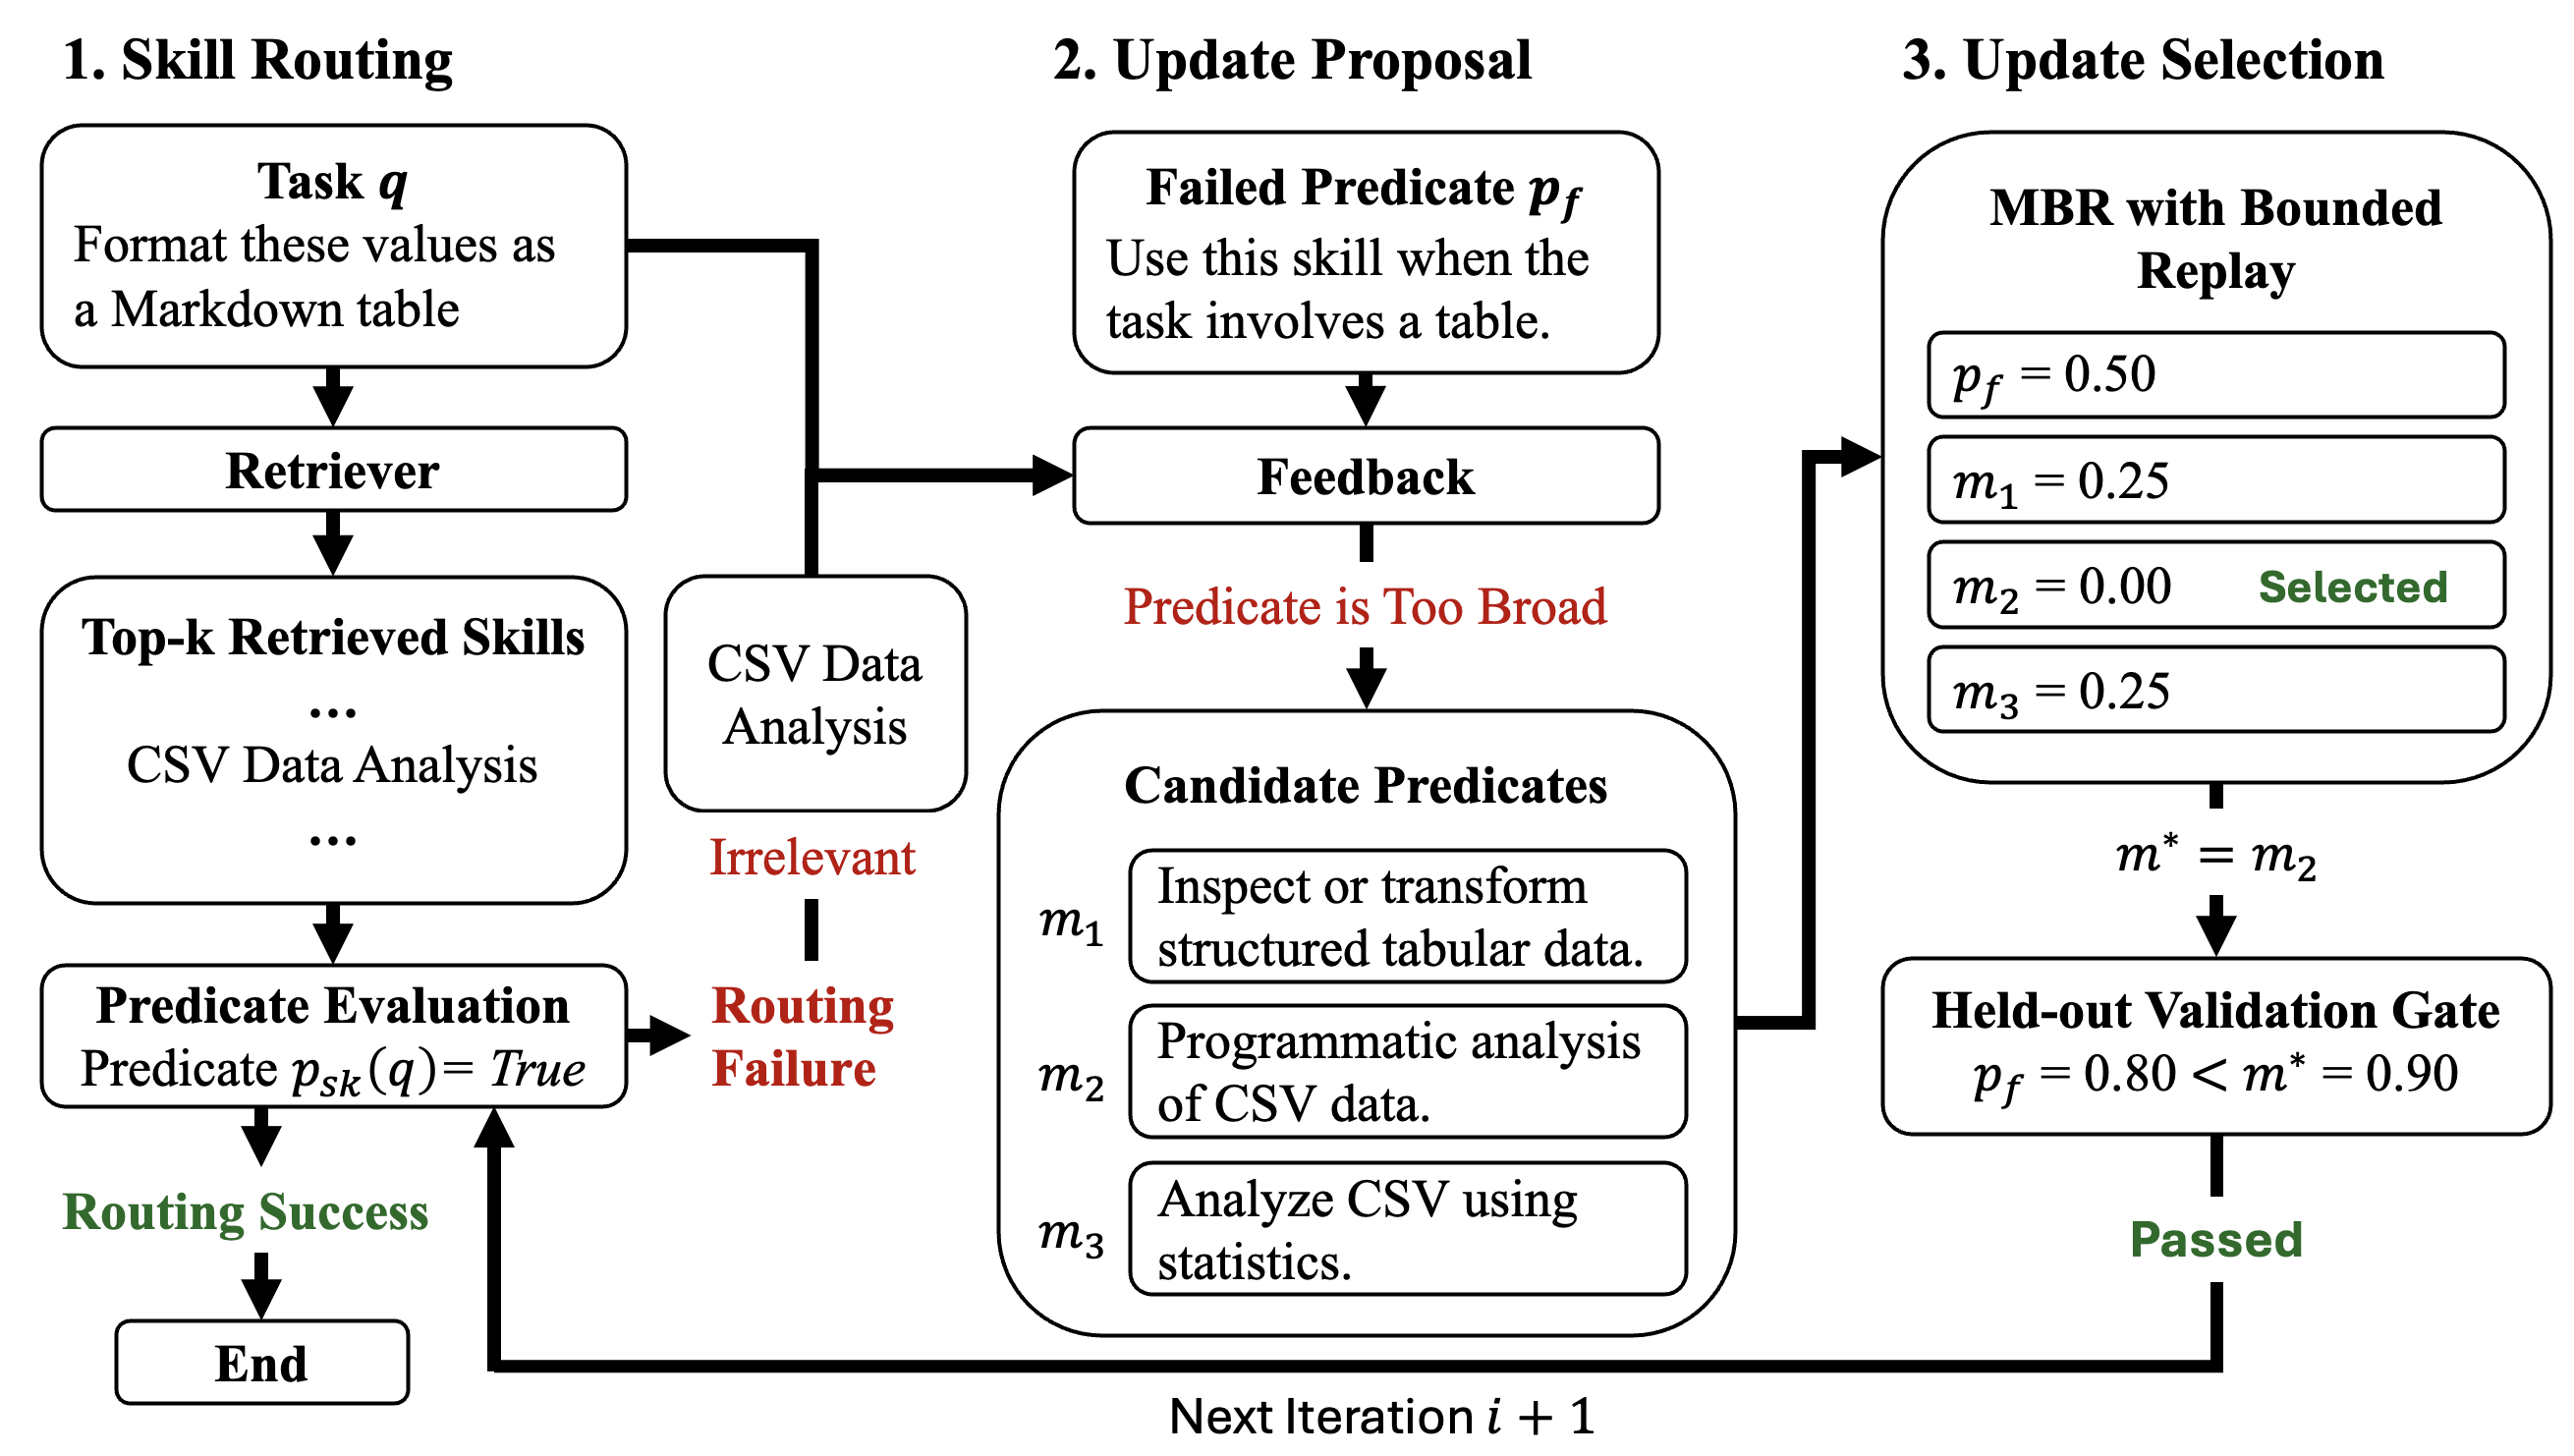
\includegraphics[width=\textwidth]{figs/method_figure.png}
\caption{RouterBSI: skill routing, predicate update proposals, and update selection with bounded replay and held-out validation.}
\label{fig:routerbsi-overview}
\end{figure*}
% INTEGRATION-END

\subsection{Non-Parametric Routing Optimization}
Non-parametric routing optimization updates external routing state from task feedback while keeping model weights fixed. Experience-based methods refine reusable memories and procedures \citep{wang2025agentworkflowmemory,ouyang2026reasoningbank}, while structural methods revise relationships among skills or tools \citep{zhang-etal-2025-toolexpnet,bai2026skilldag}. Gated methods constrain revisions through acceptance or rollback criteria \citep{pmlr-v306-mi26d,shi2026programmatic}, and JTPRO evaluates candidate updates on sampled training minibatches with held-out validation \citep{ghoshal-etal-2026-jtpro}. Nevertheless, feedback-driven revisions can disrupt earlier routing decisions, while repeatedly evaluating an expanding task history increases adaptation cost. RouterBSI addresses these challenges by selecting predicate updates through Minimum Bayes Risk over a bounded replay of relevant and irrelevant tasks, then rejects updates that increase held-out validation error.

\subsection{Parametric Routing Optimization}
Parametric routing optimization updates model weights using supervision, preferences, or execution feedback. Learned retrievers and rerankers score relevance between skills and tasks \citep{zheng2026skillrouter,wang2026skillisnotdocument}, while direct selectors predict which skill to invoke or whether invocation is needed \citep{ICLR2025_b646bdeb,chen2026skillskiplearningselective}. Reinforcement-learning policies optimize sequential skill use from downstream rewards \citep{wang2026sage,xia2026skillrl}. These approaches learn routing behavior through parameter training but encode selection criteria implicitly in model weights. RouterBSI keeps the underlying model fixed, and updates are inspectable and editable natural-language applicability predicates.

\subsection{Static Routing Without Feedback-Driven Optimization}
Static routing uses retrieval or inference-time selection mechanisms without optimizing routing criteria from task feedback. Similarity and case-based methods retrieve skills or prior cases through semantic matching \citep{wang2024voyager,guo2024dsagent}, while structured methods organize search through predefined hierarchies or skill relationships \citep{wang2026graphskill,liang2026skillnetcreateevaluateconnect}. LLM-based methods select or compose capabilities at inference time \citep{xia2026grasp,NEURIPS2024_e41efb03}. Although these approaches support task-dependent decisions, their routing criteria are not persistently revised to correct selection failures. RouterBSI uses such failures to refine skill applicability predicates online.
